\documentclass{article} % For LaTeX2e
\usepackage{nips13submit_e,times}
%\usepackage{hyperref}
\usepackage[hyphens]{url}
\usepackage{alltt}
\usepackage{multirow, caption}
\usepackage{algorithm}
\usepackage{amsmath}
\usepackage{graphicx}
\usepackage[noend]{algpseudocode}
\usepackage{etoolbox}
\usepackage{hyperref}
\usepackage{fancyvrb}
\usepackage{tgcursor}
\usepackage{amsfonts}
\usepackage[ampersand]{easylist}
\usepackage{wrapfig}
\newcommand\userinput[1]{\textbf{#1}}
\newcommand\comment[1]{\textit{#1}}
\newcommand\stdout[1]{\textsl{#1}}

\makeatletter
\preto{\@verbatim}{\topsep=0pt \partopsep=0pt }
\makeatother

\title{MapReduce Framework\\Final Report}

\author{
Derek Tzeng\\
Carnegie Mellon University\\
Pittsburgh, PA 15213 \\
\texttt{dtzeng@andrew.cmu.edu} \\
\And
Yiming Zong\\
Carnegie Mellon University\\
Pittsburgh, PA 15213 \\
\texttt{yzong@cmu.edu} \\
}

% The \author macro works with any number of authors. There are two commands
% used to separate the names and addresses of multiple authors: \And and \AND.
%
% Using \And between authors leaves it to \LaTeX{} to determine where to break
% the lines. Using \AND forces a linebreak at that point. So, if \LaTeX{}
% puts 3 of 4 authors names on the first line, and the last on the second
% line, try using \AND instead of \And before the third author name.

\newcommand{\fix}{\marginpar{FIX}}
\newcommand{\new}{\marginpar{NEW}}

\nipsfinalcopy % Uncomment for camera-ready version

\begin{document}

\maketitle

\begin{abstract}
This report reflects our final progress on MapReduce Framework project for 15-440, Fall 2014. We will first give an overview of the framework and discuss its components one by one. Then, we will describe the lifecycle of a MapReduce job and demonstrate the communication protocol between MapReduce components. Also, we will outline how to build and test the current framework from source, and include a Developer's Guide for developing MapReduce Applications based on the framework. Eventually, we will survey some additional unimplemented features that would be desirable for a commercial package.
\end{abstract}

\section{Overview of MapReduce Framework}

\par\qquad MapReduce is a highly scalable and parallel computing model that allows application programmers to specify \emph{Map} and \emph{Reduce} methods on a distributed data set in order to complete computational tasks. According to our design, nodes on the framework have one of the three following roles: \emph{Master}, \emph{Worker}, and the \emph{Users}.
\par\qquad Essentially, \emph{Master} is the coordinating node that does not store any data or perform any computational tasks but merely work on administrative tasks like maintaining a global Job Queue and a DFS Lookup Table. On the other hand, a \emph{Worker} receives and performs tasks pushed from \emph{Master}, and also holds partitions of data on the Distributed File System. Last but not least, a \emph{User} node is a designated client of the MapReduce framework, so where an end-user is able to push data on to the DFS and execute a MapReduce job based on the data.
\par\qquad Next section contains more detailed specifications of the three components.

\section{Framework Components}
\par\qquad First of all, we will show how the components of MapReduce framework relate to each other in the diagram as follows. In the digram on the next page, there is one Master node, three Worker nodes, and two User nodes.

\begin{figure}[h!]
  \caption{Sample MapReduce Framework Diagram}
  \centering
  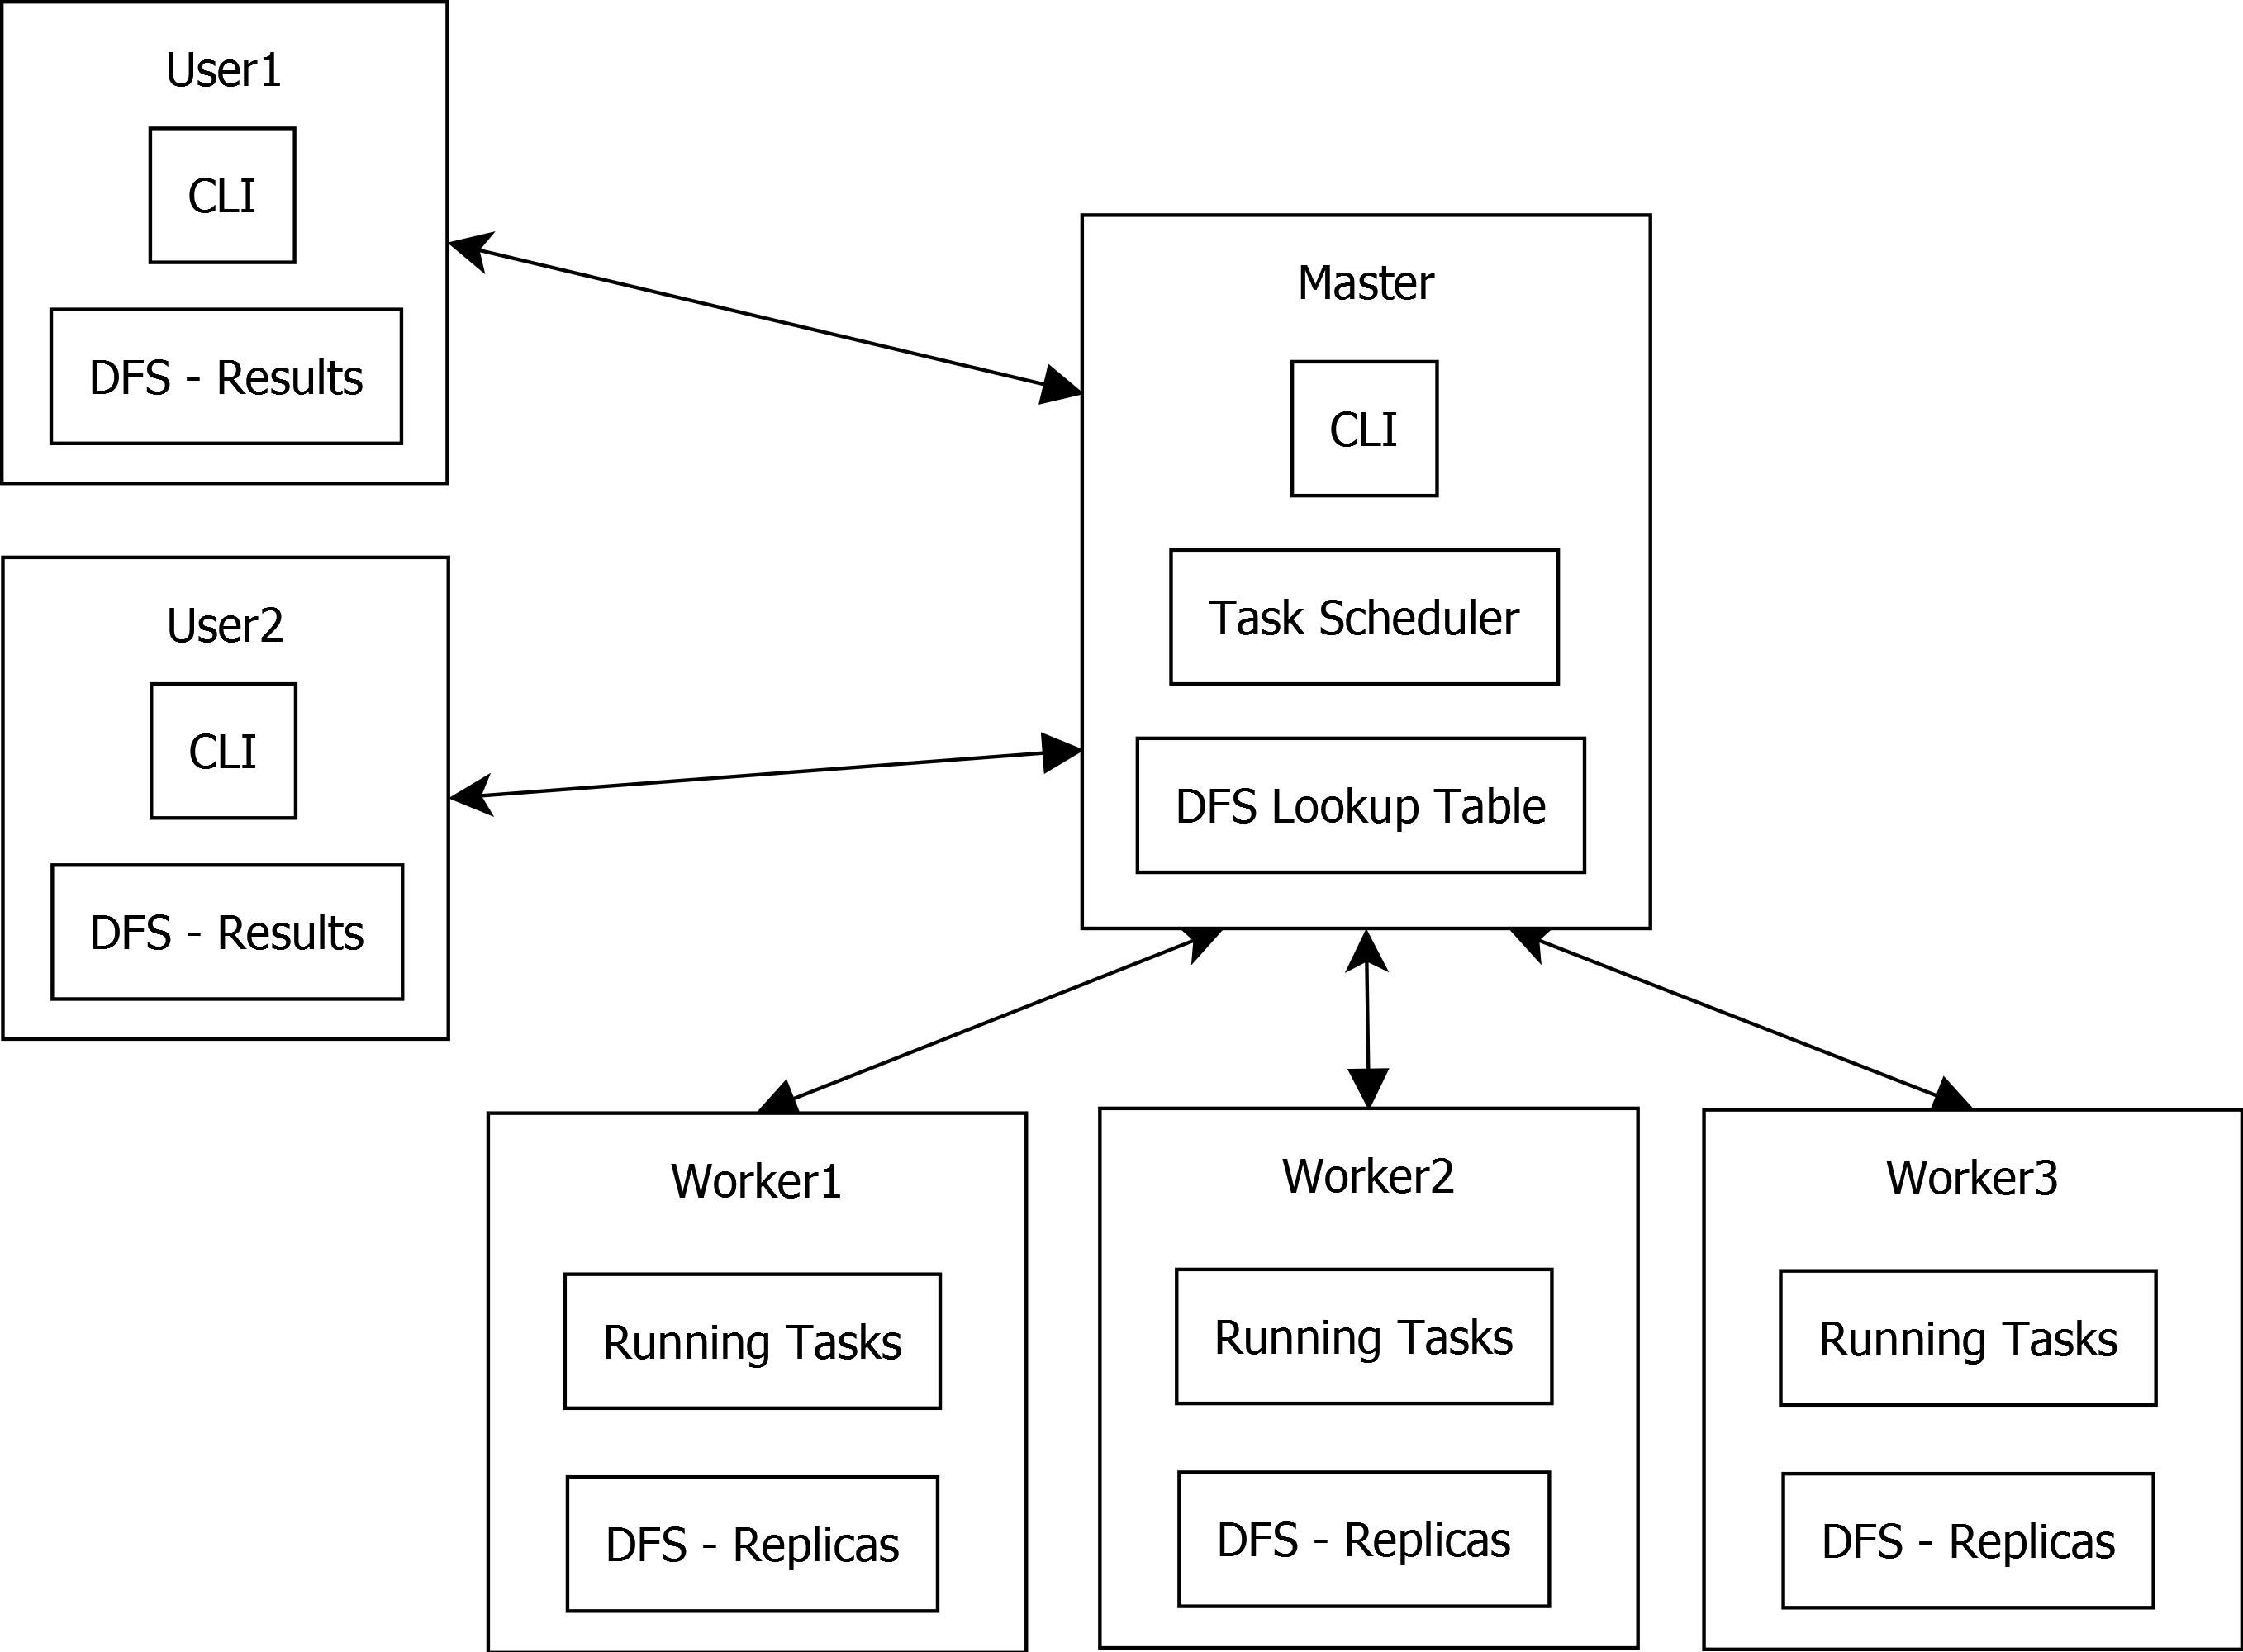
\includegraphics[width=1.05\textwidth]{design.png}
\end{figure}

\subsection{MapReduce/DFS Master}

\par\qquad The Master node, as the name suggests, is the coordinator of the frameworks. Throughout the lifecycle of a MapReduce job, it talks to both workers and users of the framework, and its main purposes include: 
\begin{easylist}[itemize]
    & Keep track of all jobs and tasks on the framework;
    & Schedule pending tasks to available slots on each;
    & Maintain look-up table of files on DFS;
    & Send heartbeat request to all workers periodically; and
    & Accept client (user) requests to add file or execute MapReduce job.
\end{easylist}

\par\qquad Meanwhile, to make the life of the system administrator a lot easier, we have included an administrative shell in our Master node, which supports the following commands:

\begin{easylist}[itemize]
    & \texttt{jobs}: Displays the list of running jobs;
    & \texttt{tasks}: Displays the list of running tasks;
    & \texttt{files}: Shows the list of files on the DFS;
    & \texttt{workers}: Displays the list of workers in the facility;
    & \texttt{users}: Shows the list of current users of facility;
    & \texttt{shutdown}: Gracefully shuts down the MapReduce facility.
\end{easylist}

\par\qquad Nonetheless, it is important to notice that our Master is a \emph{single point of failure} in our framework, because once it fails, all information related to Jobs, Tasks, and Distributed Files are lost, and recovery is impossible because we also don't know which partial results should be sent to which user client.

\subsection{MapReduce/DFS Workers}

\par\qquad The Worker nodes are the nodes in the framework that actually perform the map/reduce tasks and store partitions of files of DFS into their working directories. They are \emph{hidden} from the users, so only the Master node is able to contact with them. Since the nature of the Worker node is more \emph{daemonized} (i.e. background process that processes incoming requests from the Master), there is no command-line interface for the workers, and once we start them we leave them running, until the Master node disconnects from the network.

\subsection{MapReduce Users}

\par\qquad In our design, MapReduce users are specifically designated nodes that are allowed to interact with the MapReduce cluster by contacting the Master node. Especially, they should be able to push a local file onto the DFS for use as the input file to a MapReduce job. Similar to the Master node, we also included a user shell in each of the user nodes, which supports the following commands:

\begin{easylist}[itemize]
    & \texttt{jobs}: Displays the list of running jobs;
    & \texttt{files}: Shows the list of files on the DFS;
    & \texttt{upload <filename>}: Uploads a certain local file onto DFS;
    & \texttt{<JobName> <InputFile> <StartRecord> <EndRecord> <OutputFile> <Args>}: Executes a MapReduce job with job name \texttt{JobName}, input file \texttt{InputFile}, output file \texttt{OutputFile}, input record range \texttt{StartRecord} to \texttt{EndRecord}, and user-defined extra arguments \texttt{Args};
    & \texttt{quit}: Gracefully exits the User node.
\end{easylist}

\par\qquad Traditionally, only the Master node and Worker nodes are viewed as part of the MapReduce cluster infrastructue. In this case, we are also consider the users as a crucial component because the system administrator is able to change the list of users that are allowed to interact with a certain MapReduce infrastructue. Also, when the \emph{reduce} jobs are done, the output files are explicitly pushed to the user node. Therefore, for our framework we consider the users as a \emph{component of} the cluster, instead of as merely a client.

\section{Lifecycle of MapReduce Job}
Here is what happens when a MapReduce job is executed:
\subsection*{Step One: User Loads File onto DFS}
\par\qquad Given that the MapReduce framework is correctly initialized, the user would call \texttt{upload} command on user CLI, which sends the byte contents of the local file to the Master.  Master node takes the data and partitions it into blocks based on the \texttt{PartitionSize} parameter specified in the configuration.  For each block, the Master finds a random subset of workers (equal to \texttt{ReplicationFactor} in config), and send the partition to each of the subset of workers.  If the operations are successful, Master updates its file trackers (look-up table) and informs user that operation has succeeded.

\subsection*{Step Two: User Starts Job from User CLI}
\par\qquad When a user want to execute a MapReduce job with some file on DFS as input, the user uses the \texttt{<JobName> <InputFile> <StartRecord> <EndRecord> <OutputFile> <Args>} command on user CLI, as specified in \emph{Section 2.3}. When the parameters reach Master node, it splits the user job into \emph{map}, \emph{sort}, and \emph{reduce} tasks and adds the metadata of tasks into the scheduler. The scheduler will keep track of all the task dependencies and push the appropriate tasks to the worker nodes when they are ready to be run.

\subsection*{Step Three: Coordination Between Master and Workers to Complete Job/Tasks}
\par\qquad Master and workers must coordinate to make sure that task dependencies are reinforced while keeping track of remaining tasks for a job.  When a \emph{map} task is completed on a worker, it notifies the master, so the Master knows that its corresponding \emph{sort} task is ready to be executed anytime on the intermediate file.  Similarly, when a \emph{sort} task is completed on a worker, it also notifies the master, but the \emph{reduce} task is only ready to be launched when all \emph{sort} tasks on that specific worker are done.  Eventually, when a \emph{reduce} task is done, the final result output file has been produced, so the worker simply sends back the result file to the master, which in turn will relay the file back to the user that created the job. Therefore, the result file will end up in the user's DFS working directory.

\section{Failure Handling}
\par\qquad Due to the inherent unreliability of a network, it is not unlikely that some request packages fail to go through temporarily. Also, because potentially a large number of machines can be involved in the framework, it is fairly possible that some nodes go down while running a task. Without proper failure handling, that faulty node can be a \emph{single point of failure (SPOF)}, which is what we want to avoid in a distributed system. Therefore, we adopted the following three approaches to handle failures:
\begin{easylist}[itemize]
    & Periodic Heartbeat: The master node sends periodic \texttt{ping} requests to all workers. If after a certain amount of time the worker still has not responded, we mark the worker as ``faulty'', and migrate the tasks already assigned to it to other nodes (see \emph{Task Migration} below);
    & Task Retry: When a task fails on a node for some reason, we allow the task to be re-routed to another node for re-try before marking the task as failed. With this measure, we avoid the case when a task and a worker are not compatible -- for example, when the underlying file system of that worker node has a bad sector;
    & Task Migration: After we have determined that a node is faulty, we re-distribute all tasks running on that node to other available nodes. In this case, we do not need to restart the entire Job only because of one faulty worker node.
\end{easylist}

\section{Special Considerations}
\par\qquad Following are special features that the authors think are useful for application programmers and are beyond the request of the project specification:

\subsection{Command Line Utility at RMI Servers and Users:}
    \par\qquad Different from Hadoop's approach, our MapReduce framework comes with an interactive shell for both \emph{user} and \emph{master} nodes. The shells support most functions as currently supported by Hadoop, and the advantage is that once the shell is up, running any command is only up to the communication time within the framework. In Hadoop's approach, however, a JVM needs to be started for each MapReduce/DFS operation, e.g. \texttt{hdfs dfs -ls foobar}. We are not certain why Hadoop did not choose this approach, but our alternative approach is more light-weight and gives lower latency.
\subsection{Elegant Error Catching:}
    \par\qquad Even the best application developers in the world cannot guarantee that their first attempt at writing a complex MapReduce job will work. Therefore, when an application developer feeds us buggy code that causes exceptions in mapper, sorter, or reducer, it is important that the worker node and the Master do not abort. For our framework, when a task causes an exception, the corresponding worker thread would catch it, and send \texttt{taskFailed} to the Master. Although this handling approach can still be improved (see \emph{Section 8.3}), it does guarantee that the availability of our framework is not affected by bugs in user code.
\subsection{MapReduce Elegant Shutdown:}
    \par\qquad When the Master node in the MapReduce framework shuts down, its Workers also automatically shut down after cleaning up the working directory for DFS. Meanwhile, the \emph{User} (client) nodes are kept on, but with a message \texttt{DISCONNECTED} attached to the prompt. Also, if a \emph{User} node fails to contact Master after a period of time (defined by user), its state automatically becomes \texttt{DISCONNECTED}, and the user is also able to \emph{re-connect} with the Master. This allows the user nodes to not lose their states due to temporary connection problem to the Master node.
\subsection{Worker Failure Checking with Heartbeats:}
    \par\qquad In our implementation, there is a background heartbeat thread at Master node that keeps polling all workers nodes for their statuses. Should any node fail to respond, we give the Master a certain number of chances to retry the heartbeat (defined in user configuration file). If the worker eventually fails to respond, Master re-schedules all tasks related to the node without failing the entire MapReduce job. This makes our MapReduce framework extra resilient to worker failures.
\subsection{Designated User Nodes:}
    \par\qquad In our implementation, the user nodes are specifically listed in the configuration file, i.e. the system administrator has full control over which nodes are allowed to communicate with Master node and interact with DFS or execute MapReduce jobs. This adds an extra layer of security for the framework.


\section{Developer's Guide -- Using MapReduce Framework}

\par\qquad Since the MapReduce Framework is to be used by application developers, a pre-compiled Javadoc of the project can be found in the \texttt{doc/} directory under the project root. Users can simply open \texttt{doc/index.html} and access the documentation of the entire code base including the API usage guides. The mechanism of MapReduce Framework has been explained in previous sections.

\par\qquad In order to fit a Java Object into the MapReduce Framework, say, \texttt{WordCount}, the application programmer should create three classes: \texttt{WordCountMapper} that extends the base \texttt{Mapper} class, and similarly \texttt{WordCountSorter} and \texttt{WordCountReducer}. Then, the developer should put the classes under \texttt{mapr/examples} directory, such that MapReduce users are able to execute job based on our definition of \emph{Mapper}, \emph{Sorter}, and \emph{Reducer}.

\par\qquad In general, application developers are strongly recommended to look at the sample applications in the Package \texttt{mapr.examples}, and follow the existing code. We have provided the sample code for WordCount and Grep, and other MapReduce applications can be built similarly.

\section{Dependencies, Building, and Testing}

\par\qquad The \texttt{dtzeng.yzong} handin directory will contain two sub-directories, i.e. \texttt{reports} and \texttt{RMIFramework}. In the former directory you can find this report file, and in the latter directory is the clean source code for the project.

\subsection{Dependencies}

\par\qquad This project does not have any external dependencies, and can be compiled with standard Java libraries. To build the project from scratch without using IDE, see the following section.

\subsection{Building Instructions}

\par\qquad To build the project from scratch, use the \texttt{build.sh} script provided in the handin directory at \texttt{/afs/andrew/course/15/440-f14/handin/lab3/dtzeng-yzong.x}.

\begin{Verbatim}[commandchars=\#\[\]]
gkesden@ghc11 dtzeng-yzong.x$ #userinput[chmod +x build.sh]
gkesden@ghc11 dtzeng-yzong.x$ #userinput[./build.sh]
\end{Verbatim}

\par\qquad This will create a jar file called \texttt{MapReduce.jar}.  You may copy this jar to any desired directory for testing below.

\subsection{Testing Instructions}

\par\qquad The following test routine is designed to survey most functionalities of the MapReduce framework. Feel free to experiment with different commands in MapReduce Master and MapReduce User command-line interfaces.  In our example, our facility has 1 master and 3 workers, with 2 users connected.  First, change the hostnames in \texttt{mapr.properties} to reflect the desired Gates machines for testing.  Let \texttt{GHC\_M} be the host of the master process, \texttt{GHC\_{W1/2/3}} the workers, and \texttt{GHC\_{U1/2}} the users.

To start up the facility, do the following:

\begin{easylist}[itemize]
 & Start up master
\begin{Verbatim}[fontsize=\scriptsize, xleftmargin=-.2in,commandchars=\#\[\]]
gkesden@#comment[GHC_M] dtzeng-yzong.x$ #userinput[java -cp MapReduce.jar mapr.master.MasterCoordinator mapr.properties]
\end{Verbatim}
 & On each of the workers
\begin{Verbatim}[fontsize=\scriptsize, xleftmargin=-.2in,commandchars=\#\[\]]
gkesden@#comment[GHC_W?] dtzeng-yzong.x$ #userinput[java -cp MapReduce.jar mapr.worker.WorkerCoordinator mapr.properties worker?]
\end{Verbatim}
 && Now that the facility has started up, the command line on the master should appear.  Make sure to connect at least 1 worker to the master before the specified timeout, otherwise the facility will shutdown automatically.  With the facility started up, you can now start the 2 users.
 & On each of the users
\begin{Verbatim}[fontsize=\scriptsize, xleftmargin=-.2in,commandchars=\#\[\]]
gkesden@#comment[GHC_U?] dtzeng-yzong.x$ #userinput[java -cp MapReduce.jar mapr.user.UserCoordinator mapr.properties user?]
\end{Verbatim}
\end{easylist}

\par\qquad So, now we have everything up and running.  On the master, you can use the \texttt{workers} and \texttt{users} commands to see the status of the workers and users.  Now, let's upload our example files.  You can do this on any user.  This demonstrates on \texttt{user1}.
\begin{Verbatim}[commandchars=\#\[\]]
user1@9876 > #userinput[upload large_count.log]
File replicated successfully.
user1@9876 > #userinput[upload large_grep.log]
File replicated successfully.
\end{Verbatim}

\par\qquad Now, when you run the \texttt{files} command on either user or master, you can see the information of the files on the DFS, and where the replications are located.  Let's now start a new WordCount and Grep job.
\begin{Verbatim}[commandchars=\#\[\]]
user1@9876 > #userinput[count large_count.log 0 99999 ctr_out]
Job started with ID 0
user1@9876 > #userinput[grep large_grep.log 0 99999 grep_out tzeng]
Job started with ID 1
\end{Verbatim}
You can now use the \texttt{jobs} command on either user or master, to see the status of the job.  To see the individual tasks, use \texttt{tasks} on the master machine only.  When everything is finished, you can see the results of each job in the user's specified DFS directory, or in our case \texttt{worker1-dfs-root}.

\par Now let's see what happens when a worker fails.  Start another job, and kill a worker.
\begin{Verbatim}[fontsize=\scriptsize, xleftmargin=-.2in,commandchars=\#\[\]]
user1@9876 > #userinput[count large_count.log 0 99999 ctr_out]
Job started with ID 2
	#comment[*** Kill a worker, in this example worker 1 ***]
gkesden@#comment[GHC_W1] dtzeng-yzong.x$ #userinput[java -cp MapReduce.jar mapr.worker.WorkerCoordinator mapr.properties worker1]
Successful connection to facility master established.
#userinput[^C] gkesden@#comment[GHC_W1] dtzeng-yzong.x$
\end{Verbatim}
When you run the \texttt{jobs} command again, you will see that the status for job 2, becomes \texttt{RESTARTED AS JOB 3}.  Job 3 will now finish what job 2 requested.  If you try the "files" command, you can see that the replicas on the killed worker (worker1) are removed.
\par\qquad Lastly, to shut down the facility, use the \texttt{shutdown} command on the master CLI.  The users are not included in the facility, so another interesting feature is the "reconnect" command on the user.  If the facility is started up again (masters and workers), the user can simply try to reconnect, and it will automatically be added back into the master's state.

\section{Further Work \& Enhancements}

\par\qquad Due to time constraints, although the final product is fully functional, it still lacks many features that are desired in commercial packages (like \emph{Hadoop}), and their implementation difficulties also vary. This section will mention a selected few and discuss the difficulty for implementing them.

\subsection{MapReduce Job Priority}
    \par\qquad Currently, the MapReduce jobs in our framework are executed in a first-come-first-served basis. However, it would be nice if we could support priority-based job/task scheduling, because on a production cluster we might have a MapReduce job that takes $10$ hours to complete, yet in the mean time we might want to add a job that takes $1$ hour to complete. In the current framework, we will not get our result for the shorter job untill after $11$ hours. However, if job priority is supported, then we can set the long-running job with priority value \texttt{NORMAL}, and let the short job have priority \texttt{HIGH}. In this case, the short job will be able to run even before the long job finishes, so we can get our results faster.
    
\subsection{Pipelining MapReduce Phases}
    \par\qquad In reality, sometimes application developers might want to chain many MapReduce jobs together, i.e. feed the output of a MapReduce job directly to another MapReduce job. However, our current framework only supports sending a single MapReduce job at a time based on existing input, so in this case we need someone to wait for the reduce phase of the first MapReduce to complete before assigning the second MapReduce phase. However, this manual labor can be avoided if we can enhance our Application Developer API such that it supports pipelining many MapReduce jobs together.

\subsection{Global Logging}
    \par\qquad Despite the failure recovery techniques we implemented as in \emph{Section 4}, when an exception occurs the MapReduce job will more likely survive, but it does \emph{not} help the Application Developer to debug the application because there is no persistent logging of our framework. A helpful enhancement would be for each node in the cluster to periodically log its past activities, exceptions, and then store the logs on DFS so that the application developer (User node) is able to examine the file and debug the application.

\end{document}
